\documentclass{beamer}

\usepackage{préambule}

\begin{document}

\begin{frame}
	\begin{itemize}
		\item Donner plusieurs vecteurs égaux au vecteur $\vec{BC}$ sur la figure ci-dessous : \onslide<2-> {{\color{red}$\vec{AO}, \vec{OD}, \vec{FE}$.}}
		\item Quelle est l'image du point $F$ par la translation de vecteur $\vec{DC}$ ? \onslide<2-> {{\color{blue}$A$.}}
	\end{itemize}

	\begin{center}
		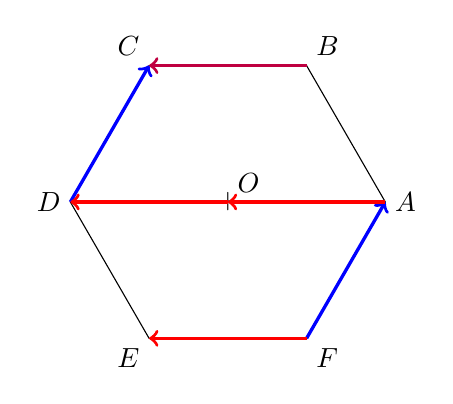
\begin{tikzpicture}
			\coordinate (O) at (0,0);
			\coordinate (A) at (2,0);
			\coordinate[rotate around={60:(O)}] (B) at (A);
			\coordinate[rotate around={120:(O)}] (C) at (A);
			\coordinate (D) at (-2,0);
			\coordinate[rotate around={60:(O)}] (E) at (D);
			\coordinate[rotate around={120:(O)}] (F) at (D);

			\foreach \p/\dir in {
					O/above right,
					A/right,
					B/above right,
					C/above left,
					D/left,
					E/below left,
					F/below right} {
					\node[\dir] at (\p) {$\p$};
				}
			\draw (A) -- (B) -- (C) -- (D) -- (E) -- (F) -- (A);
			\node at (O) {+};

			\draw<2->[very thick,purple,->] (B) -- (C);
			\draw<2->[very thick,blue,->] (D) -- (C);
			\draw<2->[very thick,blue,->] (F) -- (A);
			\foreach \a/\b in {A/O,F/E,O/D} {
					\draw<2->[very thick,red,->] (\a) -- (\b);
				}
		\end{tikzpicture}
	\end{center}
\end{frame}

\end{document}